Il serait tout à fait légitime de penser que le 
\textsf{NoSQL} soit là pour remplacer les \textsf{BDDR}
classiques. Mais ceci est difficilement imaginable de
nos jours. L’intérêt pour le \textsf{NoSQL} s'est considérablement
accru à l'issu des annonces d’adoption de ces technologies par les 
grands acteurs d'\textsf{Internet} tels 
\textsf{Google} et \textsf{Facebook} qui se sont multipliées. Ces acteurs
n'ont pas pour autant abandonné \textsf{BDDR}. \textsf{Google} et 
\textsf{Facebook} utilisent \textsf{MySQL}\cite{mysqlcustomers}.
\\
\\
Ci-dessous quelques traitements auxquels le modèle relationnel
classique ne répond pas et qui pourrait motiver le recours aux
technologies \textsf{NoSQL}\index{Limites du \textsf{SQL}}:

%% \paragraph{Indexation d'une quantité de documents:}
%% Un problème se pose quant à l'indexation d'une quantité importante de
%% données. Par exemple pour le \textsf{SGBD} \textsf{SQL Server}, la
%% version $2008$ supporte au plus $999$ indexes et chaque index, chaque
%% index peut couvrir au maximum 16 colonnes et la somme des tailles des
%% colonnes couvertes ne doit pas excéder $900\ octets$\cite{SQLserver}

\paragraph{Environnement distribué:} pour faire face à des volumes importants 
de données, il est possible de les repartir sur différentes machines physiques. 
Pour avoir plusieurs points d'accès aux données, il est nécessaire de les dupliquer
sur différents serveurs. Toutes ces opérations constituent en la mise en place d'un 
environnement distribué. Les \textsf{SGBDR} classiques montrent des limites dans un 
environnement distribué. Ces {SGBD} ne sont pas destinés à fonctionner dans un
environnement à données reparties du fait de l'opération de jointure
qui est difficilement réalisable entre des tables réparties sur des systèmes différents\cite{RickCattell}.
Les \textsf{SGBDR} classiques effectuent également des opérations impliquant de la distribution des données
mais ces opérations ne sont pas du type « \textit{shared nothing} ». Les coeurs et les processus impliqués
dans ces opérations se partagent mutuellement la \textsf{RAM} et l'espace disque mémoire.

\paragraph{Données à structure dynamique et libre:} les 
\textsf{BDDR} classiques prévoient un schéma statique à 
l'avance. Le schéma est organisé en tables de données où les lignes
contiennent les mêmes types et nombre de colonnes. Celles-ci n'offrent
donc pas un environnement dynamique pour les enregistrements. Aussi
les \textsf{SGBDR} fonctionnent avec des données structurées
organisables en tables.  Ce n'est pas le cas avec des données non
structurées, telles les données de traitement de texte et les images
\cite{NealLeavitt}.

\paragraph{Réécritures fréquentes:}  en effet, les \textsf{SGBDR} classiques en générale
appliquent la consistance forte et ce grâce aux propriétés \textsf{ACID}. 
Ces opérations sont à l'origine d'\textit{overhead} 
et sont appliquées même pour les opérations simples d'écriture dans la base. Ceci diminuera
considérablement la performance en cas de réécritures fréquentes des données même pour
les opérations simples.
Les \textsf{BDDR} mettent en avant un système d'indexation très évolué. L'utilisation
d'index est plutôt conseillée pour les systèmes où l'accès en écriture est
beaucoup plus important que celui en écriture. Tout ceci laisse penser que le modèle relationnel
classique prévoit plus de lectures que d'écritures. 

\paragraph{Extensibilité de la base:} comme signaler à la section \ref{carac}, 
la scalabilité horizontale qui est l'une des caractéristiques principales 
des solutions \textsf{NoSQL}, offre la possibilité 
d'ajouter des nœuds au cluster pour gagner en performance. Les \textsf{SGBDR} classiques 
n'ont pas cette propriété de scalabilité horizontale.
\\ 
\\ 
L'extensibilité requise, la grande quantité de données
et les mises à jour massives rendent le modèle relationnel inefficace, ce qui a
obligé à trouver un nouveau modèle. Cependant il est important de prendre en
considération quelques aspects au risque d'une mauvaise utilisation. «
L'intérêt d'une base de données \textsf{NoSQL} pour un projet ne
dépend pas du volume de données qu'elle aura à manipuler. Le choix de
son utilisation doit être basé sur la préférence d’un mode de
représentation et non sur une forte volumétrie
»\cite{NoSQLeurope}. Il ne s’agit donc pas d’une solution
miracle pour tout type de stockage de données.  La tentative de
reproduire dans une base de données \textsf{NoSQL} une représentation
ou un comportement habituellement offert par la représentation en tables
n'aboutira pas à une solution plus efficace car l'architecture des 
\textsf{SGBDR} y est exclusivement destinée.
%Dan McCreary a également convenu avec Michael Stonebraker que les
%utilisateurs NoSQL ne partagent pas un langage de requête unifiée, ce
%qui va ralentir l'adoption de NoSQL\cite{SergeLeblal}.
\\
\\
À présent, je vais attirer l'attention sur une différence fondamentale
entre ces deux familles de gestionnaires de données. Elles n'ont pas
la même conception de la gestion des données. Le \textsf{SQL} impose
un format de stockage le plus explicite possible à l'utilisateur pour
permettre au gestionnaire d'avoir la maîtrise totale des données
stockées afin d'en assurer l'intégrité. Le gestionnaire \textsf{SQL}
ne se contente pas uniquement de répondre aux requêtes. Il effectue
d'autres opérations qui consistent en l'entretien de la base à l'image
de \textsf{MySQL} dont 96\% des cycles machines sont de
l'\textit{overhead}. Le \textsf{NoSQL} vise à éviter les opérations
d'\textit{overhead} afin de consacrer toutes les ressources machines
aux seuls traitements des requêtes pour être plus rapide. Cependant
la cohérence dans la \textsf{BDD} nécessite beaucoup d'apport
extérieur pour pallier à la très grande souplesse du système.  Une
illustration de cette différence philosophique entre les
deux familles de gestionnaires est la suivante:
\begin {figure}[H]
       \centering
        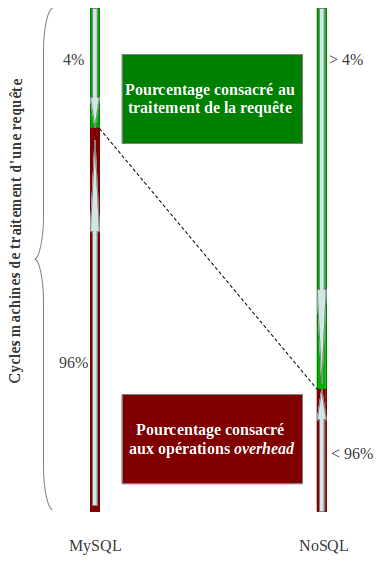
\includegraphics[scale=0.3]{\DIR/img/SQLvsNoSQL.png}	
        \caption{Répartitions des cycles machines \textsf{SQL} et \textsf{NoSQL}}
	\label{sqlvsnoql}
  \end {figure}    
\noindent
Toujours en quête de performance et comme mentionné à la section \ref{carac}, 
le \textsf{NoSQL} a renoncé à de la « \textsf{consistance forte} » pour de la « \textsf{consistance éventuelle} ». Il justifie ce choix par le théorème de \textsf{CAP} pendant que les \textsf{SGBDR} défendent systématiquement toutes les propriétés \textsf{ACID} dont la « \textsf{consistance forte} ». Ceci n'est pas sans compromis, notamment 
pour la reprise sur erreurs. 
\textsf{Michael Stonebraker} explique clairement sur 8 cas d'erreur,  
les enjeux du choix
des propriétés \textsf{CAP}\cite{MichaelStonebraker2}. Je me limiterai seulement à
3 cas d'erreur. Le but étant de mettre en relief les limites d'une « \textsf{consistance éventuelle} »
et d'exhiber deux situations qui rendent impossible la propriété \textsf{A} de \textsf{CAP} défendue par la mouvance \textsf{NoSQL}.
%===========================================================
%     Illustration enjeux du choix de AP dans CAP
%===========================================================
\def\exempleA{We assume a typical hardware model of a
collection of local processing and storage nodes assembled into a cluster using LAN networking.
The clusters, in turn, are wired together using WAN networking.
Let’s start with a discussion of what causes errors in databases:}

\def\exemple{Dans l'illustration qu'il a utilisé, \textsf{Michael Stonebraker} a considéré un ensemble de clusters interconnectés via un réseau \textsf{WAN}. 
Les nœuds à l'intérieur d'un cluster utilisent le \textsf{LAN} pour échanger. Ci-dessous trois cas d'erreur possibles:}

\def\casaA{Application errors. The application performed one or more incorrect updates. Generally, this is
not discovered for minutes to hours thereafter. The database must be
backed up to a point before the offending transaction(s), and
subsequent activity redone.}

\def\casa{Erreur au niveau de la couche application. Une application effectue une ou plusieurs mises à jour incorrectes. De telles erreurs ne sont généralement pas détectées dans les minutes qui suivent afin de revenir sur une version précédente de la base avant les mises à jour incorrectes.}

\def\casbA{Repeatable DBMS errors. The DBMS crashed at a processing node. Executing the same
transaction on a processing node with a replica will cause the backup
to crash. These errors have been termed Bohr bugs.}

\def\casb{Les erreurs reproductibles. Par exemple, une transaction fait planter le serveur principal. 
La même transaction fait tomber tous les autres serveurs copies qui vont servir de relais. 
Ces erreurs sont connues sous le nom de « \textsf{Bohr bugs} ».}

\def\cascA{\sf A disaster. The local cluster is wiped out by a flood, earthquake, etc. The cluster no longer exists.}

\def\casc{\sf Une catastrophe. Un cluster local est entièrement détruit.}

\def\commentA{First, note that errors 1 and 2 will cause problems with any high availability scheme. In these two
scenarios, there is no way to keep going; i.e., availability is
impossible to achieve. Also, replica consistency is meaningless; the
current DBMS state is simply wrong. Error 7 will only be recoverable
if a local transaction is only committed after the assurance that the
transaction has been received by another WAN-connected cluster. Few
application builders are willing to accept this kind of
latency. Hence, eventual consistency cannot be guaranteed, because a
transaction may be completely lost if a disaster occurs at a local
cluster before the transaction has been successfully forwarded
elsewhere. Put differently, the application designer chooses to suffer
data loss when a rare event (such as a disaster) occurs, because the
performance penalty for avoiding it is too high.}

\def\comment{Les deux premiers cas d'erreur conduisent la base dans un état incohérent. Ils affectent la disponibilité des données. Dans de telles situations, il est impossible de garantir la disponibilité des données même après avoir renoncé à de la consistance forte. Le troisième cas d'erreur montre les limites de
la consistance éventuelle. Les données ne pourront être récupérées que
si la transaction a été propagée sur un autre cluster avant la
catastrophe. Le temps de latence imposé par la consistance éventuelle
entre les mises à jour est donc problématique.}

\begin{center}
\begin{tabular}{p{1.7cm} p{12cm}}
\multicolumn{2}{p{14cm}}{\sf \exemple}\\&\\  
{\bf Cas 1} & \textsf{\casa}\\~&~\\ {\bf Cas 2}
& \textsf{\casb}\\~&~\\ {\bf Cas 3} & \textsf{\casc}\\
\end{tabular}
\end{center}
\noindent \comment
\\
\\
Pour finir, un paramètre à prendre en compte et pour ainsi reprendre la pensée de \textsf{Ted Dziuba},
est que contrairement aux solutions \textsf{NoSQL}, les \textsf{SGBDR} sont matures et ont par conséquent 
``une liste de limitations et de bugs connus''\cite{DieNosql}. L'utilisateur d'une \textsf{SGBDR} classique 
est plus ou moins rassuré parce qu'il sait à quoi s'en tenir. 
